\documentclass{article}
\usepackage[utf8]{inputenc} % Permite usar caracteres en español y otros idiomas

% --- PAQUETES ESENCIALES ---
\usepackage[utf8]{inputenc} % Permite usar caracteres en español y otros idiomas
\usepackage[T1]{fontenc}    % Mejora la codificación de fuentes
\usepackage{graphicx}       % Para incluir imágenes
\usepackage{amsmath}        % Fórmulas matemáticas avanzadas
\usepackage{amssymb}        % Símbolos matemáticos
\usepackage{geometry}       % Para ajustar los márgenes
\usepackage{authblk}        % Para manejar autores y afiliaciones
\usepackage{abstract}       % Para un entorno de abstract adecuado
\usepackage{hyperref}       % Para crear hipervínculos (en DOIs, URLs, etc.)
\usepackage[numbers,sort&compress]{natbib}
\usepackage{subcaption}     % Para subfiguras
\usepackage{caption}        % Para un mejor control de las captions
\usepackage{float}          % Para un mejor control de la posición de figuras con [H]
\usepackage{tikz}           % Para dibujar el diagrama del pipeline
\usetikzlibrary{positioning, arrows.meta, calc}
\usepackage{xcolor}
\usepackage{soul}
\usepackage{colortbl}   % for \rowcolor in tables
% Revision markup: \textcolor{red}{} = yellow highlight (new/changed text, soul pkg)
%                 \textcolor{blue}{} = blue text (changes containing \cite or math)

% --- CONFIGURACIÓN DE LA PÁGINA Y ESTILO ---
% Márgenes similares a los de un journal
\geometry{
    a4paper,
    total={170mm,257mm},
    left=20mm,
    top=20mm,
}

% Configuración de hyperref para que los links se vean bien
\hypersetup{
    colorlinks=true,
    linkcolor=blue,
    filecolor=magenta,      
    urlcolor=blue,
    citecolor=blue,
}

% --- BIBTEX BIBLIOGRAPHY (printed at the end) ---

% --- INFORMACIÓN DEL TÍTULO, AUTORES Y AFILIACIONES ---
\title{\textbf{Advanced Machine Learning Strategies for Predicting Therapy Response in Preclinical Glioblastoma using Longitudinal MRI}}

\author[1]{Javier González}
\author[2,3*]{Ana Paula Candiota}
\author[1,3,4*]{Alfredo Vellido}

\affil[1]{\small Department of Computer Science, Universitat Politècnica de Catalunya (UPC), Barcelona, Spain}
\affil[2]{\small Department of Biochemistry and Molecular Biology, Universitat Autònoma de Barcelona (UAB), Cerdanyola del Vallès, Spain}
\affil[3]{\small Centro de Investigación Biomédica en Red en Bioingeniería, Biomateriales y Nanomedicina (CIBER-BBN), Madrid, Spain}
\affil[4]{\small Intelligent Data Science and Artificial Intelligence (IDEAI) Research Center, UPC, Barcelona, Spain}
\affil[*]{\small \textcolor{red}{Corresponding authors: \texttt{alfredo.vellido@upc.edu} and \texttt{AnaPaula.Candiota@uab.cat}}}

% Quita la fecha para que no aparezca en el título
\date{}

%%%%%%%%%%%%%%%%%%%%%%%%%%%%%%%%%%%%%%%%%%%%%%%%%%%%%%%%%%%%%%%%%%%%%%%%%%%%%%%%
% --- COMIENZO DEL DOCUMENTO ---
%%%%%%%%%%%%%%%%%%%%%%%%%%%%%%%%%%%%%%%%%%%%%%%%%%%%%%%%%%%%%%%%%%%%%%%%%%%%%%%%

\begin{document}

\maketitle % Crea el bloque del título

% --- ABSTRACT ---
\begin{abstract}
Glioblastoma (GB) is the most aggressive primary brain tumor, characterized by a poor prognosis, limited response to therapy, and high rates of recurrence. Early therapeutic response assessment is challenging due to phenomena such as pseudoresponse and pseudoprogression. This study explores the potential of advanced machine learning (ML) strategies to predict long-term therapy outcomes using longitudinal T2-weighted Magnetic Resonance Imaging (MRI) data from a preclinical GL261 glioblastoma mouse model, acquired prior and during treatment. We compare two distinct approaches: a classical pipeline based on radiomic features coupled with an XGBoost classifier, and a deep learning (DL) pipeline using a fine-tuned EfficientNetB0 model. Our results demonstrate that while the radiomics approach identifies interpretable imaging biomarkers and achieves good predictive performance \textcolor{red}{(AUC $\approx$ 0.77, 95\% CI 0.70--0.83)}, the DL-based model outperforms it across \textcolor{red}{most} evaluation metrics, reaching an AUC of \textcolor{red}{0.868 (95\% CI 0.812--0.918)} and a sensitivity of \textcolor{red}{0.818}. The DL model shows better generalization across individual subjects, and \textcolor{red}{discriminative performance improves progressively throughout the follow-up period for both approaches}. Interpretability analysis via Grad-CAM confirms that the DL model's predictions are driven by anatomically relevant features. These findings \textcolor{red}{suggest that DL, enhanced by transfer learning, has the potential to serve as a powerful non-invasive tool} for the early prediction of treatment efficacy in glioblastoma, paving the way for more robust and personalized therapy monitoring.
\end{abstract}

% --- CUERPO DEL ARTÍCULO ---

\section{Introduction}

Glioblastoma (GB) stands as the most common and lethal primary brain tumor in adults, with a median survival of just 15-18 months despite aggressive multimodal treatment consisting of surgery, radiotherapy, and chemotherapy with temozolomide (TMZ), dating from more than two decades ago \cite{Stupp2005}. A major clinical challenge is the accurate and early assessment of treatment response. Standard evaluation criteria can be confounded by treatment-related effects such as pseudoprogression (transient, treatment-induced inflammation mimicking tumor growth) and pseudoresponse (transient decrease in the contrast enhancement area) \cite{shukla2017advanced}, which complicates clinical decision-making in early scenarios.

Preclinical models, such as the murine GL261 glioblastoma model \cite{Liu2021,Wu2020}, offer a controlled environment to study tumor evolution and response to therapy. Longitudinal Magnetic Resonance Imaging (MRI) in these models provides a rich source of data to develop and validate non-invasive biomarkers that could be later translated to clinical settings.

In recent years, Artificial Intelligence (AI) has shown great promise in medical image analysis. Two dominant paradigms have emerged: radiomics-based machine learning (ML) and deep learning (DL). Radiomics involves the high-throughput extraction of quantitative, handcrafted features from medical images, which describe tumor shape, intensity, and texture \cite{kumar2012radiomics}. These features can provide interpretable insights but rely on domain-specific feature engineering. In contrast, DL, particularly with Convolutional Neural Networks (CNNs), learns relevant hierarchical features directly from raw image data, often achieving superior performance but at the cost of reduced interpretability \cite{Hosny2018,Tran2021,Shen2017}. Despite the rapid adoption of DL, radiomics remains attractive because handcrafted features offer greater interpretability and can provide biologically meaningful descriptors of tumor morphology and heterogeneity. Consequently, direct comparisons between radiomics-based and DL-based frameworks remain important for understanding the trade-off between predictive performance and model interpretability.

This study aims to systematically compare these two approaches for the early prediction of long-term therapy outcomes (cure vs. relapse) in a preclinical GB model using longitudinal T2-weighted MRI, one of the workhorse sequences used in the MR-based scenario. We developed and evaluated both a classical radiomics-based pipeline and a modern DL-based pipeline, focusing on three key objectives:
\begin{enumerate}
    \item To assess and compare the predictive performance of both methodologies.
    \item To identify key imaging biomarkers associated with treatment response and relapse.
    \item To explore the interpretability of both models to ensure potential clinical relevance.
\end{enumerate}

By doing so, we seek to determine which of the studied strategies offers a more robust and scalable solution for developing non-invasive tools to improve glioblastoma therapy assessment.

In this context, the term \textit{longitudinal} refers to the acquisition of multiple MRI examinations from the same animal at different time points throughout tumor evolution and treatment, rather than to a single cross-sectional acquisition. This design provides information about the temporal dynamics of tumor response. It is important to note, however, that although the data are longitudinal, they were not modeled as a multivariate time series in the sense of jointly classifying complete temporal sequences \cite{Prinzi2024}. Instead, each imaging time point was treated as an individual observation, and temporal context was captured through the multi-time-point structure of the GLOO cross-validation scheme, while preserving the subject-level structure of the data during validation.

\subsection*{Related Work}
ML and DL approaches have become increasingly important in neuro-oncology, particularly for the analysis of MRI data \cite{Pitarch24}. Traditional radiomics pipelines transform medical images into quantitative descriptors of tumor morphology, intensity, and texture, enabling predictive modeling using machine learning algorithms \cite{kumar2012radiomics,pyradiomics}. Recent evidence continues to support the prognostic value of MRI-derived radiomic biomarkers in glioblastoma, although challenges related to reproducibility, feature stability, and external validation remain important barriers to clinical translation \cite{PMID:38668068}. Despite the rapid adoption of DL methods, radiomics remains attractive because handcrafted features offer greater interpretability and can provide biologically meaningful descriptors of tumor morphology and heterogeneity. Consequently, direct comparisons between radiomics-based and DL-based frameworks remain important for understanding the trade-off between predictive performance and model interpretability.

More recently, DL methods have demonstrated the ability to learn hierarchical image representations directly from imaging data, reducing dependence on handcrafted feature engineering and achieving state-of-the-art performance in several neuroimaging tasks \cite{Hosny2018,Shen2017,Tran2021,Dorfner2025}. Recent reviews have further highlighted the growing role of DL in glioblastoma imaging, where convolutional neural networks are increasingly capable of extracting clinically relevant information directly from MRI data without explicit feature engineering \cite{biomedicines12081878}.

Most existing studies have focused on tumor detection, segmentation, or diagnostic classification. For example, Cinar and Yildirim proposed a hybrid ResNet50-based architecture for brain tumor detection from MRI, achieving high classification accuracy and demonstrating the effectiveness of convolutional neural networks for neuroimaging applications \cite{Cinar2020}. However, predicting therapeutic response remains considerably more challenging because it requires longitudinal analysis and the identification of subtle imaging changes that precede overt anatomical alterations.

Several studies have explored this problem in preclinical GB models. Núñez et al. combined radiomics, Convex-NMF decomposition, and feature-selection strategies to characterize treatment effects in GL261 glioblastoma using multimodal MRI and magnetic resonance spectroscopic imaging (MRSI) data, demonstrating the potential of quantitative imaging biomarkers for therapy assessment \cite{interpretingLuisMiguel}. Ortega-Martorell et al. subsequently introduced one-dimensional convolutional neural networks for analyzing longitudinal spectroscopic data, achieving improved discrimination between responsive and non-responsive tumor regions and highlighting the capacity of DL to identify early therapy-related changes \cite{Ortega-Martorell2023}. In parallel, Zhao et al. integrated MR-based metabolomics with molecular profiling of the tumor microenvironment, linking imaging biomarkers to immune-related mechanisms associated with tumor progression and relapse \cite{Zhao2023}. Prinzi et al. further demonstrated the value of explicitly modeling radiomic features as multivariate time series in dynamic contrast-enhanced breast MRI \cite{Prinzi2024}, an approach conceptually related to, but methodologically distinct from, the time-point-based strategy adopted here.

Although these studies have demonstrated the feasibility of imaging-based response monitoring, most rely on spectroscopic imaging, multimodal acquisitions, or highly specialized biomarkers. Comparatively fewer investigations have examined whether standard T2-weighted MRI alone contains sufficient information to predict long-term therapeutic outcomes. The present study addresses this gap by directly comparing a radiomics-based ML framework with a transfer-learning DL approach for predicting relapse and cure from longitudinal T2-weighted MRI acquired in a preclinical GL261 glioblastoma model.

\section{Results}

\subsection{Performance Comparison}

Table \ref{tab:all_models} summarizes the performance of the best-performing radiomics and DL models under the Grouped Leave-One-Out (GLOO) evaluation framework.

The fine-tuned EfficientNetB0 achieved the highest overall performance, with an AUC of \textcolor{red}{0.868 (95\% CI 0.812--0.918)}, compared with \textcolor{red}{0.801 (95\% CI 0.733--0.866)} for the frozen feature-extraction configuration (EfficientNet FE+XGB) and \textcolor{red}{0.770 (95\% CI 0.703--0.832)} for the radiomics pipeline. Improvements were observed across \textcolor{red}{most} evaluation metrics, particularly sensitivity: in the fine-tuned EfficientNet configuration, \textcolor{red}{81.8\% of cured \textbf{examinations}} were correctly identified, compared with \textcolor{red}{60.6\%} for FE+XGB and \textcolor{red}{54.5\%} for XGBoost. \textcolor{red}{All metrics reported in Table~\ref{tab:all_models} are computed at the level of individual MRI examinations (exam-level); subject-level (animal-level) metrics are discussed below. A DeLong test \cite{DeLong1988} confirmed that the AUC superiority of EfficientNet FT over radiomics is statistically significant (Z\,=\,$-$4.68, $p < 0.001$), whereas the difference between EfficientNet FE+XGB and radiomics did not reach significance (Z\,=\,$-$1.31, $p = 0.19$; see Supplementary Methods for test details).}

\textcolor{red}{The radiomics model achieved higher specificity (0.810 vs.\ 0.759 for FT), reflecting a more conservative prediction tendency. In contrast, the fine-tuned DL model achieved substantially higher sensitivity (0.818 vs.\ 0.545) and NPV (0.936 vs.\ 0.862). The highest PPV was obtained by EfficientNet FE+XGB (0.541), while the radiomics model had the lowest (0.450), consistent with its tendency to classify borderline cases as relapsing. The frozen feature-extraction configuration occupied an intermediate position overall, with the highest specificity (0.853) but substantially lower sensitivity (0.606) than FT.}

% --- TABLA DE RESULTADOS ---
\begin{table*}[ht]
\centering
\small
\begin{tabular}{lcccccc}
\hline
Model & Accuracy & AUC & Sensitivity & Specificity & PPV & NPV \\
\hline

\rowcolor{red!20}
Radiomics + XGBoost &
0.748 & 0.770 & 0.545 & 0.806 & 0.444 & 0.862 \\
\rowcolor{red!20}
\textcolor{gray}{\scriptsize [95\% CI]} &
\textcolor{gray}{\scriptsize [0.698, 0.799]} &
\textcolor{gray}{\scriptsize [0.703, 0.832]} &
\textcolor{gray}{\scriptsize [0.421, 0.667]} &
\textcolor{gray}{\scriptsize [0.755, 0.856]} &
\textcolor{gray}{\scriptsize [0.338, 0.554]} &
\textcolor{gray}{\scriptsize [0.815, 0.907]} \\[2pt]

\rowcolor{red!20}
EfficientNet FE + XGB &
\textbf{0.799} & 0.801 & 0.606 & \textbf{0.853} & \textbf{0.541} & 0.884 \\
\rowcolor{red!20}
\textcolor{gray}{\scriptsize [95\% CI]} &
\textcolor{gray}{\scriptsize [0.752, 0.842]} &
\textcolor{gray}{\scriptsize [0.733, 0.866]} &
\textcolor{gray}{\scriptsize [0.486, 0.725]} &
\textcolor{gray}{\scriptsize [0.807, 0.897]} &
\textcolor{gray}{\scriptsize [0.424, 0.653]} &
\textcolor{gray}{\scriptsize [0.839, 0.923]} \\[2pt]

\rowcolor{red!20}
EfficientNet FT &
0.772 & \textbf{0.868} & \textbf{0.818} & 0.759 & 0.491 & \textbf{0.936} \\
\rowcolor{red!20}
\textcolor{gray}{\scriptsize [95\% CI]} &
\textcolor{gray}{\scriptsize [0.721, 0.819]} &
\textcolor{gray}{\scriptsize [0.812, 0.918]} &
\textcolor{gray}{\scriptsize [0.719, 0.907]} &
\textcolor{gray}{\scriptsize [0.703, 0.813]} &
\textcolor{gray}{\scriptsize [0.398, 0.583]} &
\textcolor{gray}{\scriptsize [0.899, 0.968]} \\

\hline
\end{tabular}
\caption{\textcolor{red}{Exam-level} performance comparison under GLOO cross-validation \textcolor{red}{(N=298 examinations, 10 animals)}. Bold: highest value per column. FE: frozen feature extractor; FT: fine-tuned. PPV: positive predictive value; NPV: negative predictive value. \textcolor{red}{Bootstrap 95\% CIs (10,000 resamples) shown in grey. DeLong test: FT vs.\ Radiomics $Z=-4.68$, $p<0.001$; FE+XGB vs.\ Radiomics $Z=-1.31$, $p=0.19$. EfficientNet FT is the recommended model: despite EfficientNet FE achieving a similar AUC (0.801), FT provides substantially higher sensitivity (0.818 vs.\ 0.606) and NPV (0.936 vs.\ 0.884), the clinically most relevant metrics for identifying cured animals.}}
\label{tab:all_models}
\end{table*}

\subsection{Radiomics Model Analysis}

Progressive refinement of the radiomics pipeline revealed the importance of rigorous feature selection in high-dimensional imaging datasets. Models trained using the complete feature set exhibited unstable behavior and reduced generalization, whereas statistical filtering and redundancy removal substantially improved predictive performance. A comparison of the resampling strategies evaluated for the XGBoost classifier is reported in Supplementary Figure S1.

The baseline configuration, trained on the full feature set, achieved high specificity but poor sensitivity, effectively defaulting to a relapse prediction under the strong class imbalance. Because correctly identifying cured animals was the primary objective, subsequent configurations targeted sensitivity while preserving specificity. \textcolor{red}{In the final configuration, all feature selection steps (variance filter, Spearman correlation filter, Mann--Whitney $U$ test, and heuristic filter retaining only original image-derived features) were applied exclusively within the training partition of each GLOO fold, so that no information from the held-out test animal contaminated any preprocessing or selection decision. On average, $21.7 \pm 1.8$ features were selected per fold (range 18--25) from the initial set of 1,218. This procedure yielded an exam-level AUC of 0.770 (95\% CI: 0.703--0.832) and a sensitivity of 0.545.}

\textcolor{red}{At the animal level, majority-vote aggregation across all examinations per subject produced AUC values of 0.92, 0.92 and 0.88 for radiomics, EfficientNet FE+XGB and EfficientNet FT, respectively, with specificity of 1.00 across all three pipelines (no relapsing animal misclassified). EfficientNet FT correctly identified four of five cured animals, compared with three of five for the other two configurations. The two cured animals consistently misclassified across all pipelines (C1285 and C1382) showed mean predicted cure probabilities below 0.50 throughout the follow-up, suggesting that their imaging signatures overlap substantially with those of relapsing animals. Detailed per-animal predictions for all three models are provided in Supplementary Table~S5.}

Feature importance analysis consistently identified a small subset of descriptors as dominant contributors to classification decisions across folds. The top-ranked features were Elongation, Dependence Non-Uniformity Normalized, Long Run High Gray Level Emphasis, and Run Entropy. These features collectively describe tumor morphology (Elongation, Major Axis Length), spatial heterogeneity of gray-level dependencies (Dependence Non-Uniformity Normalized), intensity-run texture patterns (Long Run High Gray Level Emphasis), and complexity of gray-level sequences (Run Entropy). The temporal evolution of Elongation and Dependence Entropy — a closely related GLDM descriptor reflecting spatial complexity — across the follow-up is illustrated in Figures~\ref{fig:elongation} and~\ref{fig:dependenceentropy} as representative examples of features that differentiate the two groups.

Longitudinal analysis revealed distinct temporal trajectories between cured and relapsing tumors. In cured animals, Elongation (Figure \ref{fig:elongation}) progressively decreased following treatment administration, whereas relapsing tumors maintained more irregular growth patterns throughout follow-up.

\begin{figure}[H]
\centering
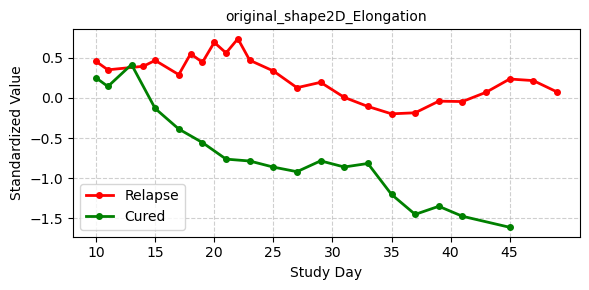
\includegraphics[width=0.6\linewidth]{images/elongation.png}
\caption{Elongation value evolution across cured and relapse groups.}
\label{fig:elongation}
\end{figure}

Dependence Entropy (Figure \ref{fig:dependenceentropy}) increased in cured animals during the later stages of treatment, while remaining comparatively stable in relapsing animals.

\begin{figure}[H]
\centering
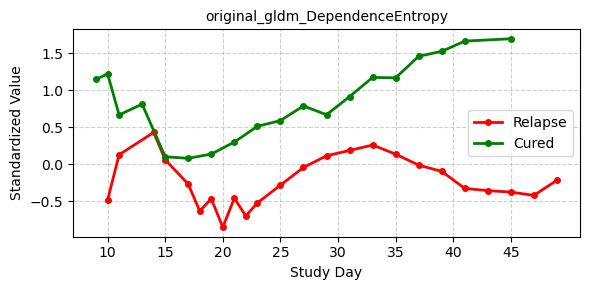
\includegraphics[width=0.6\linewidth]{images/dependenceentropy.png}
\caption{Dependence Entropy evolution across cured and relapse groups.}
\label{fig:dependenceentropy}
\end{figure}

The repeated identification of these descriptors across the different feature-selection strategies supports their robustness within the present cohort. \textcolor{red}{These longitudinal trajectories are presented as illustrative group-level tendencies within five animals per group and should not be interpreted as statistically established biomarkers; formal repeated-measures testing and independent validation in larger cohorts would be required to confirm them.} Additional low-dimensional visualizations of the selected radiomic feature space (t-SNE and UMAP projections) are provided in Supplementary Figure S2.

\subsection{Deep Learning Model Analysis}

Among all evaluated architectures and training configurations, the fine-tuned EfficientNetB0 model trained exclusively on grayscale MRI images achieved the best overall performance, with \textcolor{red}{an AUC of 0.868 (95\% CI 0.812--0.918), an accuracy of 77.2\%, and a sensitivity of 81.8\%}.

\textcolor{red}{Performance improved consistently along the transfer-learning axis. Training from scratch without mask information performed worst (AUC 0.5331); adding binary tumor masks raised discrimination substantially (AUC 0.7699); initializing from ImageNet weights provided a further boost, with the frozen feature-extraction configuration reaching an AUC of 0.801 (95\% CI 0.733--0.866); and end-to-end fine-tuning produced the most balanced classifier (AUC 0.868, 95\% CI 0.812--0.918, sensitivity 0.818, NPV 0.936). This ordering indicates that both pre-trained representations and full fine-tuning were the main drivers of performance.}

The inclusion of tumor masks as additional input channels did not improve the fine-tuned model and occasionally reduced predictive accuracy. This result indicates that, given sufficient training capacity, the network was able to identify relevant regions directly from the MRI data without explicit localization guidance.

\subsection{Temporal Prediction Performance}

\textcolor{red}{Predictive accuracy improved progressively throughout tumor evolution for all three pipelines. Stratified analysis by examination time point (early: day $\leq$21, mid: day 22--31, late: day $>$31) yielded the following exam-level AUC values:}

\begin{table}[H]
\centering
\textcolor{red}{
\begin{tabular}{lccc}
\hline
Model & Early ($\leq$21\,d) & Mid (22--31\,d) & Late ($>$31\,d) \\
\hline
Radiomics + XGBoost & 0.582 & 0.809 & 0.960 \\
EfficientNet FE+XGB & 0.741 & 0.767 & 0.987 \\
EfficientNet FT      & 0.788 & 0.902 & 1.000 \\
\hline
\end{tabular}
}
\caption{\textcolor{red}{Temporal stratification of AUC by tercile of day of study (N=101 early, 100 mid, 97 late examinations).}}
\label{tab:temporal}
\end{table}

\textcolor{red}{These results indicate that radiomics performance is near-chance in early treatment (AUC~0.58), whereas both DL configurations maintain substantially higher discrimination from the earliest time points (AUC~0.74--0.79). Claims of reliable early prediction for the radiomics model should be interpreted cautiously; the DL models, particularly EfficientNet FT (early AUC 0.788), show a more consistent temporal profile. All three models approach or reach excellent discrimination at late time points (AUC~0.96--1.00).}

\textcolor{red}{For the radiomics pipeline, misclassifications were concentrated in the earliest study days (approximately days 9--21), especially for cured animals, whose imaging signatures became distinctive only as therapeutic effects accumulated.} The per-day distribution of classification accuracy and misclassified examinations is reported in Supplementary Figure S3.

\subsection{Interpretability and Error Analysis}

Gradient-weighted Class Activation Mapping (Grad-CAM) visualizations showed that EfficientNet predictions were predominantly driven by anatomically meaningful regions (Figure \ref{fig:day11}). In correctly classified cases, attention maps consistently highlighted the tumor core and its immediate surroundings, and frequently extended into peritumoral regions.

\begin{figure}[H]
    \centering
    \begin{subfigure}[b]{0.32\textwidth}
        \centering
        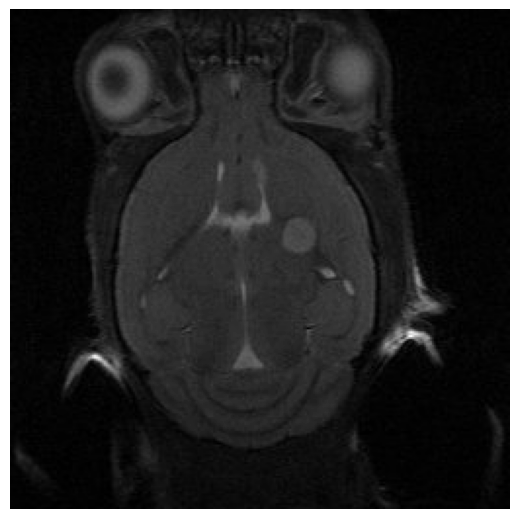
\includegraphics[width=\textwidth]{images/1263_d11_mri.png}
        \caption{D11 - MRI}
        \label{fig:1263_d11_mri}
    \end{subfigure}
    \hfill
    \begin{subfigure}[b]{0.32\textwidth}
        \centering
        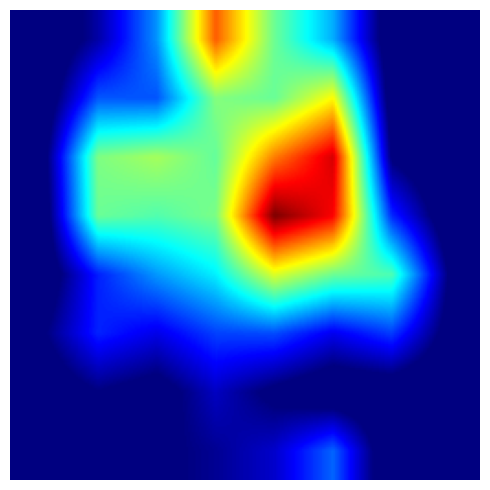
\includegraphics[width=\textwidth]{images/1263_d11_heat.png}
        \caption{D11 - Heatmap}
        \label{fig:1263_d11_heat}
    \end{subfigure}
    \hfill
    \begin{subfigure}[b]{0.32\textwidth}
        \centering
        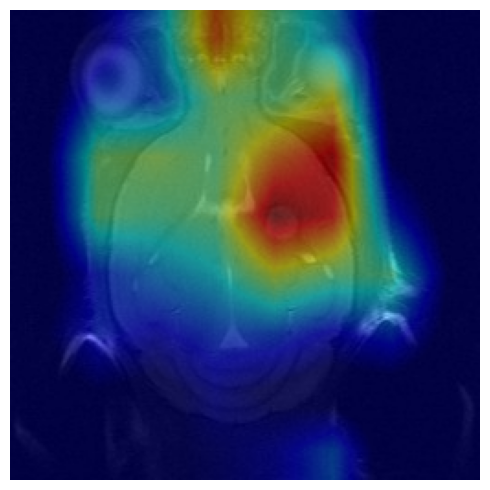
\includegraphics[width=\textwidth]{images/1263_d11_gradcam.png}
        \caption{D11 - Grad-CAM}
        \label{fig:1263_d11_gradcam}
    \end{subfigure}
    \caption{Day 11 visualization for subject C1263 (correctly predicted): original MRI, Grad-CAM heatmap, and Grad-CAM overlay. The temporal evolution of these maps across days 14, 17, and 19 is shown in Supplementary Figure S4.}
    \label{fig:day11}
\end{figure}

Analysis of misclassified examinations revealed a different pattern: model attention frequently shifted toward anatomically irrelevant structures or became spatially diffuse. Tracking a representative relapsing subject (C1263) across consecutive time points illustrates this behavior: on the correctly classified Day 11 the attention was centered on the tumor, whereas on Day 14 the saliency map became diffuse and misaligned, on Day 17 it focused on the animal's eye---an artifact-related region with no pathological significance---and on Day 19 it again failed to localize the tumor. Prediction failures were thus associated with uncertainty regarding lesion localization rather than an inability to learn discriminative tumor features. The evolution of Grad-CAM attention maps across these consecutive time points is provided in Supplementary Figure S4.


\section{Discussion}
This study investigated whether longitudinal T2-weighted MRI contains imaging signatures capable of predicting long-term therapeutic outcome in a preclinical GL261 glioblastoma model, \textcolor{red}{within the framework of a proof-of-concept study based on a small but well-characterized cohort of 10 treated animals.} Two complementary strategies were evaluated: a radiomics-based ML pipeline using handcrafted quantitative descriptors and an image-based deep learning framework built upon transfer learning. Although both approaches demonstrated predictive capability, the DL model achieved superior performance across \textcolor{red}{most} evaluation metrics, suggesting that image-derived representations capture relevant information that is not fully represented by conventional radiomic features. \textcolor{red}{The effective number of independent observations in this study is 10 subjects, and all reported metrics should be interpreted in this light; the wide bootstrap confidence intervals (e.g., AUC 95\% CI 0.703--0.832 for radiomics) reflect this inherent statistical limitation.}

The radiomics approach successfully identified several interpretable imaging biomarkers whose temporal behavior differed between cured and relapsing tumors \textcolor{red}{in the studied cohort}. Elongation reflects the geometric anisotropy of the lesion, and its progressive reduction in cured animals is consistent with the development of a more compact and structurally homogeneous tumor following successful therapy; in contrast, the persistently irregular morphology observed in relapsing tumors may indicate ongoing infiltrative growth. Texture-based descriptors such as Run Entropy and Dependence Entropy quantify the complexity and heterogeneity of spatial intensity distributions, where elevated values generally reflect greater local variability and structural disorder. The increase in Dependence Entropy observed in cured animals during later treatment stages may reflect tissue-remodeling processes, inflammatory responses, or treatment-induced structural reorganization occurring after tumor regression. This trend---increasing entropy associated with a favorable outcome---is an illustrative descriptive observation based on five cured animals and should be regarded as hypothesis-generating rather than as an established biomarker; independent confirmation in larger cohorts would be required before any translational conclusion can be drawn. These observations are consistent with previous radiomics studies demonstrating that texture heterogeneity carries prognostic information beyond conventional anatomical measurements, and they suggest that therapeutic response is accompanied by progressive microstructural changes detectable before substantial anatomical differences become apparent.

The superior sensitivity of the fine-tuned DL model \textcolor{red}{(0.818 exam-level; 0.800 animal-level)} suggests that convolutional networks can capture more complex and subtle spatial patterns than handcrafted radiomic features\textcolor{red}{, although this finding merits investigation in a larger cohort, more representative of biological variability. A DeLong test confirmed that the AUC advantage of EfficientNet FT over radiomics is statistically significant at the examination level ($Z=-4.68$, $p<0.001$); the difference between EfficientNet FE+XGB and radiomics was not significant ($p=0.19$), indicating that end-to-end fine-tuning is the key driver of improved discrimination rather than the use of ImageNet representations per se.} \textcolor{red}{It should be noted, however, that both pipelines process each MRI examination independently without explicitly modeling the longitudinal sequence; temporal context is encoded in the radiomics pipeline through engineered descriptors, but neither approach constitutes a sequence model in the strict sense.} \textcolor{red}{The PPV of the radiomics model (0.450) is low, reflecting the class imbalance and the small cohort; in a realistic clinical setting where long-term cures are rarer than in this controlled preclinical model, PPV would be expected to be substantially lower, and these results should be interpreted as a proof-of-concept demonstration rather than as evidence of clinical deployability.} The success of transfer learning from a model pre-trained on natural images (ImageNet) underscores its value in overcoming data scarcity, a pervasive challenge in preclinical medical imaging: general-purpose low-level filters were effectively adapted to the specific task of identifying predictive patterns in T2-weighted MRI scans. Notably, the finding that explicit tumor masks did not improve performance, and could even degrade it, indicates that treatment-response signatures are likely distributed across both tumor and peritumoral tissue, rather than confined to the manually segmented lesion \textcolor{red}{in the studied cases}. This is coherent with the Grad-CAM analysis, in which attention frequently extended into peritumoral regions.

These results are aligned with, and extend, previous work on preclinical glioblastoma. Núñez et al. \cite{interpretingLuisMiguel} and Ortega-Martorell et al. \cite{Ortega-Martorell2023} demonstrated the value of radiomics and one-dimensional convolutional networks applied to multimodal MRI/MRSI data, while Zhao et al. \cite{Zhao2023} linked MR-based metabolomic signatures to immune-related mechanisms of relapse. Our findings \textcolor{red}{suggest} that a substantial fraction of the response-related information can already be recovered from standard T2-weighted MRI alone, without spectroscopic or multimodal acquisitions. In contrast to approaches that model radiomic dynamics as a jointly classified multivariate time series \cite{Prinzi2024}, we treated each time point as an individual observation while encoding temporal context through engineered descriptors and subject-aware validation; this design is better suited to the irregular and heterogeneous sampling of our cohort.

Although DL models are frequently criticized as ``black boxes'', the Grad-CAM analysis demonstrates that their decisions can be interpreted and that correct predictions are consistently associated with anatomically relevant attention. Conversely, misclassifications were associated with diffuse or anatomically irrelevant attention, suggesting that errors stem primarily from uncertainty in lesion localization rather than from a failure to learn discriminative features. \textcolor{red}{The temporal stratification (Table~\ref{tab:temporal}) reveals a consistent pattern across all three pipelines: discriminative performance is lowest in the early treatment window and improves markedly at later time points. Radiomics shows the steepest improvement (AUC 0.582 early to 0.960 late), while the DL pipelines achieve substantially higher early-window AUCs (EfficientNet FE+XGB: 0.741; EfficientNet FT: 0.790). This indicates that DL models, benefiting from richer image representations, can extract meaningful predictive signals even before treatment effects have fully accumulated, although performance remains highest at later time points for all models. Claims of reliable early prediction for radiomics remain limited; for the DL models, particularly EfficientNet FT, early-window performance is encouraging but should be confirmed in larger cohorts.}

Several limitations should be considered when interpreting these results. First, the study was conducted using a relatively small cohort of 18 animals, which restricts statistical power and may limit generalizability. \textcolor{red}{Accordingly, these results should be interpreted with caution, as a preliminary proof-of-concept, pending confirmation in future studies with larger and more biologically diverse cohorts.} Although Grouped Leave-One-Out validation was employed to minimize information leakage and provide a realistic estimate of model performance, larger independent cohorts will be necessary to confirm the robustness of the identified biomarkers.

Second, all analyses were performed using a single preclinical glioblastoma model (GL261) and data acquired at a single institution. While the GL261 model reproduces several important biological characteristics of human glioblastoma, additional validation in alternative experimental models and clinical datasets will be required before translational conclusions can be drawn.

Third, the radiomics pipeline relied on manual tumor segmentations, introducing potential observer-dependent variability. Automated or semi-automated segmentation approaches may improve reproducibility in future studies.

Finally, only T2-weighted MRI was analyzed. The incorporation of additional imaging modalities, including diffusion MRI, perfusion imaging, spectroscopy, or multimodal radiomic signatures, may provide complementary information and further improve predictive performance.

\section{Conclusion}

\textcolor{red}{We have demonstrated, as a proof-of-concept in a well-characterized preclinical cohort of 10 treated animals, that both radiomics and DL have the potential to become viable strategies for predicting therapy outcomes in preclinical glioblastoma from longitudinal T2-weighted MRI. A DL approach based on fine-tuning a pre-trained EfficientNetB0 outperforms the classical radiomics pipeline across most evaluation metrics, achieving the highest AUC (0.868, 95\% CI 0.812--0.918), sensitivity (0.818 exam-level; 0.800 animal-level) and NPV (0.936). The difference in AUC over radiomics is statistically significant (DeLong $Z=-4.68$, $p<0.001$). The fine-tuned model was selected as the recommended configuration over the frozen feature extractor (AUC 0.801) because it provides substantially higher sensitivity (0.818 vs.\ 0.606) and NPV (0.936 vs.\ 0.884), better supporting the primary clinical goal of identifying cured animals. The DL model's discriminative ability, combined with interpretable Grad-CAM attention maps, makes it a promising candidate for non-invasive biomarker development. Temporal analysis reveals that predictive performance improves substantially over the follow-up period, with the most reliable signal available after approximately three weeks; early-window predictions should therefore be treated with appropriate caution. This work provides a solid foundation, fostering future research aimed at creating more reliable and personalized methods for monitoring glioblastoma treatment, once confirmed in larger cohorts representing biological variability.}

Future work should focus on external validation, multimodal integration, and longitudinal modeling. In particular, combining conventional MRI with spectroscopic, metabolic, molecular, or histopathological information may provide a more comprehensive representation of tumor evolution. Furthermore, temporal DL architectures capable of explicitly modeling sequential imaging examinations could better exploit the longitudinal nature of therapeutic response. Such developments may ultimately pave the way for clinically deployable systems for early treatment adaptation and personalized glioblastoma management.

\section{Materials and Methods}

An overview of the two analytical pipelines evaluated in this study is presented in Figure \ref{fig:pipeline}. Their details are provided in the following subsections.

\begin{figure}[H]
\centering
\resizebox{0.52\textwidth}{!}{%
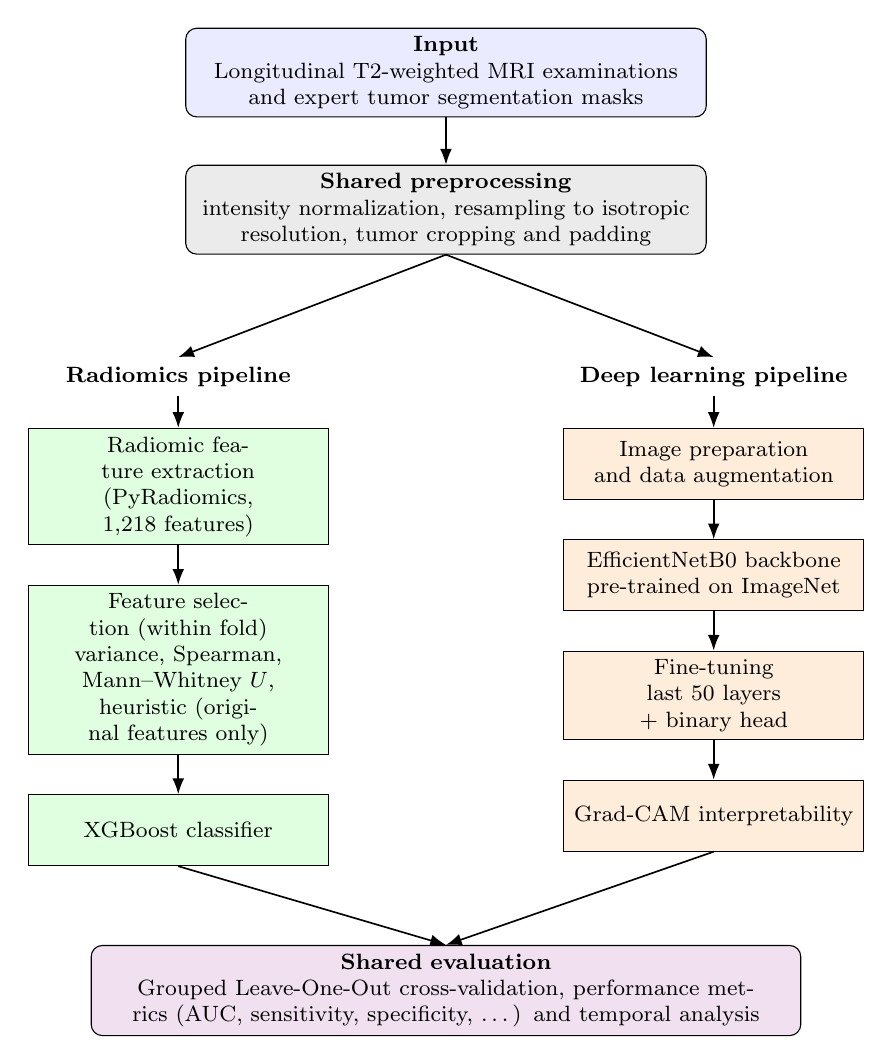
\begin{tikzpicture}[
    font=\footnotesize,
    io/.style={rectangle, rounded corners, draw, fill=blue!8, text width=6.4cm, minimum height=9mm, align=center, inner sep=3pt},
    pre/.style={rectangle, rounded corners, draw, fill=black!8, text width=6.4cm, minimum height=9mm, align=center, inner sep=3pt},
    rad/.style={rectangle, draw, fill=green!12, text width=3.6cm, minimum height=9mm, align=center, inner sep=3pt},
    dnn/.style={rectangle, draw, fill=orange!14, text width=3.6cm, minimum height=9mm, align=center, inner sep=3pt},
    ev/.style={rectangle, rounded corners, draw, fill=violet!12, text width=8.8cm, minimum height=9mm, align=center, inner sep=3pt},
    ttl/.style={font=\footnotesize\bfseries},
    ar/.style={-{Latex[length=2mm]}, semithick}
]
\node[io] (input) {\textbf{Input}\\ Longitudinal T2-weighted MRI examinations\\ and expert tumor segmentation masks};
\node[pre, below=6mm of input] (pre) {\textbf{Shared preprocessing}\\ intensity normalization, resampling to isotropic resolution, tumor cropping and padding};

\node[rad, below=22mm of pre, xshift=-34mm] (r1) {Radiomic feature extraction\\ (PyRadiomics, 1{,}218 features)};
\node[rad, below=5mm of r1] (r2) {Feature selection (within fold)\\ variance, Spearman, Mann--Whitney $U$,\\ heuristic (original features only)};
\node[rad, below=5mm of r2] (r4) {XGBoost classifier};

\node[dnn, below=22mm of pre, xshift=34mm] (d1) {Image preparation\\ and data augmentation};
\node[dnn, below=5mm of d1] (d2) {EfficientNetB0 backbone\\ pre-trained on ImageNet};
\node[dnn, below=5mm of d2] (d3) {Fine-tuning\\ last 50 layers + binary head};
\node[dnn, below=5mm of d3] (d4) {Grad-CAM interpretability};

\node[ttl, above=4mm of r1] (rt) {Radiomics pipeline};
\node[ttl, above=4mm of d1] (dt) {Deep learning pipeline};

\node[ev, below=10mm of r4, xshift=34mm] (ev) {\textbf{Shared evaluation}\\ Grouped Leave-One-Out cross-validation, performance metrics (AUC, sensitivity, specificity, \dots) and temporal analysis};

\draw[ar] (input) -- (pre);
\draw[ar] (pre.south) -- (rt.north);
\draw[ar] (pre.south) -- (dt.north);
\draw[ar] (rt) -- (r1);
\draw[ar] (dt) -- (d1);
\draw[ar] (r1) -- (r2);
\draw[ar] (r2) -- (r4);
\draw[ar] (d1) -- (d2);
\draw[ar] (d2) -- (d3);
\draw[ar] (d3) -- (d4);
\draw[ar] (r4.south) -- (ev.north);
\draw[ar] (d4.south) -- (ev.north);
\end{tikzpicture}%
}
\caption{Overview of the experimental workflow. Longitudinal T2-weighted MRI examinations and their corresponding tumor masks share a common preprocessing stage and are then processed through two parallel pipelines: a radiomics-based pipeline coupled with an XGBoost classifier and a deep learning pipeline based on a fine-tuned EfficientNetB0 model. Both pipelines are evaluated under the same Grouped Leave-One-Out cross-validation scheme.}
\label{fig:pipeline}
\end{figure}

\subsection{Preclinical Dataset}

This study used a retrospective dataset of longitudinal T2-weighted (T2w) MRI scans acquired from 18 C57BL/6 mice orthotopically implanted with GL261 GB cells and monitored throughout tumor evolution \cite{Wu2020}. These tumor-bearing mice were either control/untreated or treated with TMZ following an immune-enhancing metronomic schedule \cite{Wu2015}. The animals were divided into three outcome groups:
\begin{itemize}
    \item \textbf{Control (n=8):} untreated mice, showing natural tumor progression.
    \item \textbf{Relapsing (n=5):} mice treated with TMZ that showed a transient response followed by tumor regrowth.
    \item \textbf{Cured (n=5):} mice treated with TMZ that showed complete tumor regression and long-term survival.
\end{itemize}

The dataset is longitudinal in nature: each animal underwent a variable number of imaging examinations acquired at different time points along tumor evolution, so that the number of explorations and the range of days studied differ across subjects (Figure \ref{fig:temporal}). A summary of the cohort is presented in Table \ref{tab:cohort}, and a detailed per-subject description (number of images per exploration, number of explorations, and range of days studied) is provided in Supplementary Table S1.

\begin{figure}[H]
\centering
\resizebox{!}{7.5cm}{%
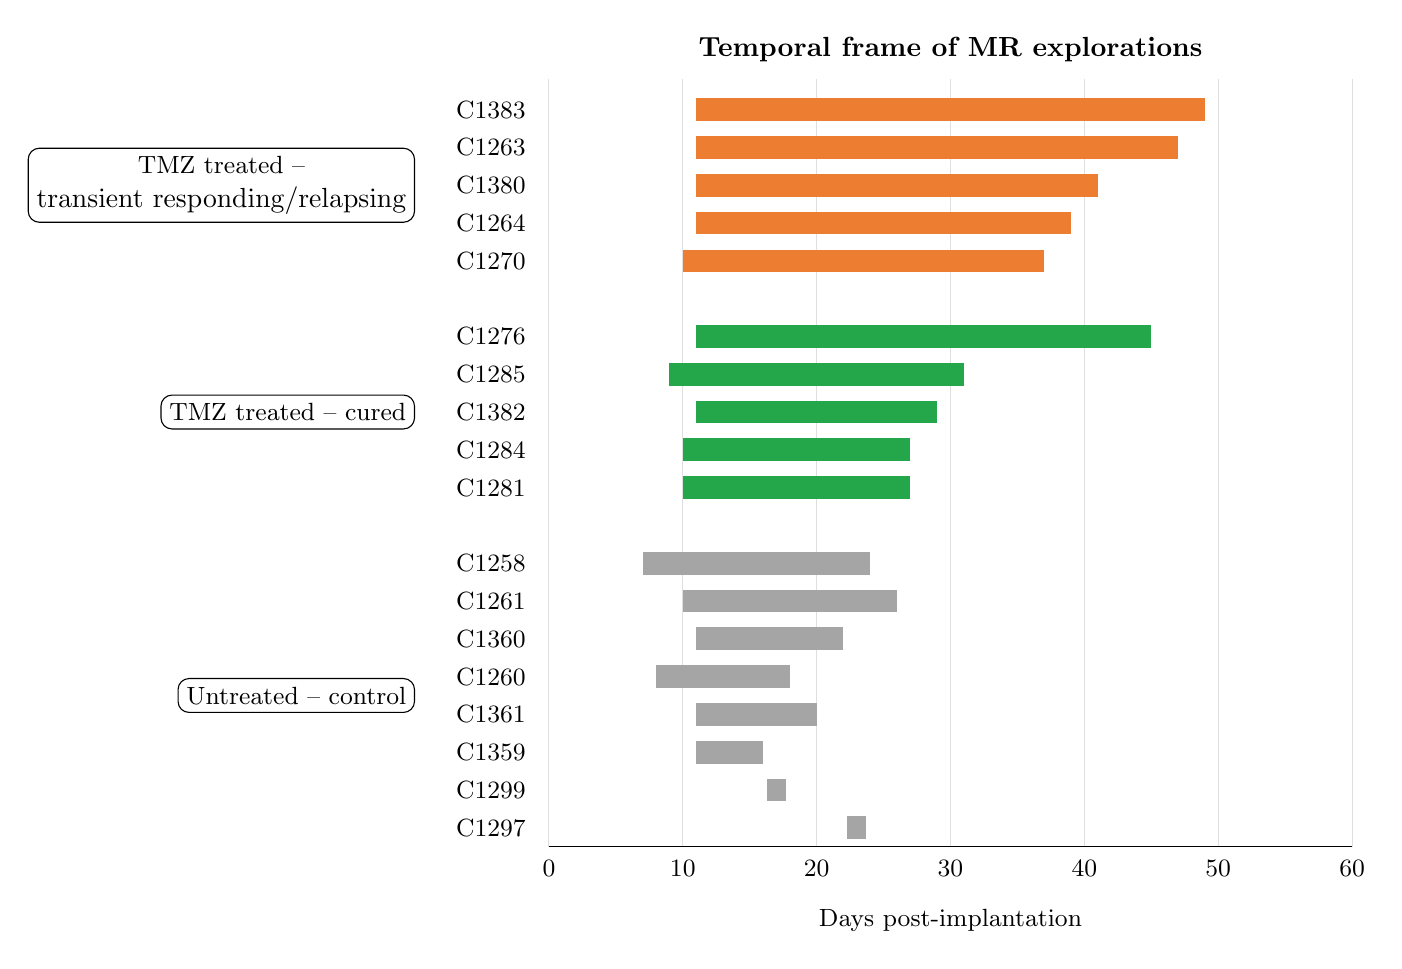
\begin{tikzpicture}[x=0.17cm, y=0.48cm]
    \definecolor{grprelapse}{RGB}{237,125,49}
    \definecolor{grpcured}{RGB}{35,167,74}
    \definecolor{grpcontrol}{RGB}{165,165,165}
    % title
    \node[font=\bfseries] at (30,21.6) {Temporal frame of MR explorations};
    % vertical grid and x-axis ticks
    \foreach \d in {0,10,20,30,40,50,60}{
        \draw[gray!25] (\d,0.5) -- (\d,20.8);
        \node[anchor=north] at (\d,0.4) {\small \d};
    }
    \draw (0,0.5) -- (60,0.5);
    \node[anchor=north] at (30,-0.9) {\small Days post-implantation};
    % bars: y / start / end / color / label
    \foreach \y/\s/\e/\c/\lab in {%
        20/11/49/grprelapse/C1383, 19/11/47/grprelapse/C1263,
        18/11/41/grprelapse/C1380, 17/11/39/grprelapse/C1264,
        16/10/37/grprelapse/C1270,
        14/11/45/grpcured/C1276, 13/9/31/grpcured/C1285,
        12/11/29/grpcured/C1382, 11/10/27/grpcured/C1284,
        10/10/27/grpcured/C1281,
        8/7/24/grpcontrol/C1258, 7/10/26/grpcontrol/C1261,
        6/11/22/grpcontrol/C1360, 5/8/18/grpcontrol/C1260,
        4/11/20/grpcontrol/C1361, 3/11/16/grpcontrol/C1359%
    }{
        \fill[\c] (\s,\y-0.3) rectangle (\e,\y+0.3);
        \node[anchor=east] at (-1,\y) {\small \lab};
    }
    % single-exploration controls (points)
    \foreach \y/\d/\lab in {2/17/C1299, 1/23/C1297}{
        \fill[grpcontrol] (\d-0.7,\y-0.3) rectangle (\d+0.7,\y+0.3);
        \node[anchor=east] at (-1,\y) {\small \lab};
    }
    % group labels
    \node[anchor=east, align=center, draw, rounded corners, inner sep=3pt]
        at (-10,18) {\small TMZ treated --\\ transient responding/relapsing};
    \node[anchor=east, align=center, draw, rounded corners, inner sep=3pt]
        at (-10,12) {\small TMZ treated -- cured};
    \node[anchor=east, align=center, draw, rounded corners, inner sep=3pt]
        at (-10,4.5) {\small Untreated -- control};
\end{tikzpicture}%
}
\caption{Temporal frame of the MRI explorations for each animal in the cohort. Each horizontal bar spans the range of days post-implantation over which a given subject (CXXXX) was imaged, grouped by experimental condition: TMZ-treated transient responding/relapsing (orange), TMZ-treated cured (green), and untreated control (grey). Day~0 corresponds to the tumor inoculation day; subjects C1297 and C1299 underwent a single exploration. Per-subject details are reported in Supplementary Table~S1.}
\label{fig:temporal}
\end{figure}

The animal experiments from which these data were obtained were approved by the Ethics Committee on Animal Experimentation (CERec) of the Universitat Autòno\-ma de Barcelona (protocols CEA-OH-9685 and CEEAH-3665), and conducted in accordance with the 3Rs principles (Replacement, Reduction, and Refinement), Spanish legislation (Real Decreto 53/2013), and European Directive 2010/63/EU on the protection of animals used for scientific purposes.

Imaging was performed on a 7T Bruker BioSpec 70/30 USR spectrometer (Bruker BioSpin GmbH, Ettlingen, Germany), equipped with a mini-imaging gradient set (400 mT/m). A 72-mm inner-diameter linear volume coil was used as a transmitter, and a dedicated mouse brain quadrature surface coil was used as a receiver. Mice were positioned in a bed, which allowed delivery of anaesthesia (isoflurane, 1.5–2.0\% in O2 at 1 L/min), with an integrated heating water circuit for body temperature regulation. Respiratory frequency was monitored with a pressure probe and kept between 60–80 breaths/min. GB-bearing mice were screened with high-resolution coronal T2w MRI using a Rapid Acquisition with Relaxation Enhancement (RARE) sequence to evaluate the presence of brain tumors and monitor their stage of evolution, with repetition time (TR)/effective echo time (TEeff) = 4200/36 ms. For each MRI scan, tumor regions were manually segmented by experts to create binary masks. The core analysis focused on discriminating between the "Cured" and "Relapsing" groups to specifically model treatment-response dynamics. {\color{black}\sethlcolor{yellow}\textcolor{red}{Animals were monitored daily by trained veterinary personnel according to a standardized welfare scoring system aimed at assessing animal well-being and detecting signs of tumour progression. The scoring system evaluated several clinical and behavioural criteria. A body weight loss exceeding 20\% of the initial weight was considered a predefined humane endpoint and led to euthanasia. Animals were then euthanized by cervical dislocation under isoflurane anaesthesia, as described above.}} 

A representative example of the longitudinal acquisition is shown in Figure \ref{fig:longitudinal}, which illustrates consecutive T2-weighted examinations of a single treated animal together with the corresponding expert tumor segmentations across several time points.

\begin{figure}[H]
\centering
\begin{subfigure}[b]{\textwidth}
\centering
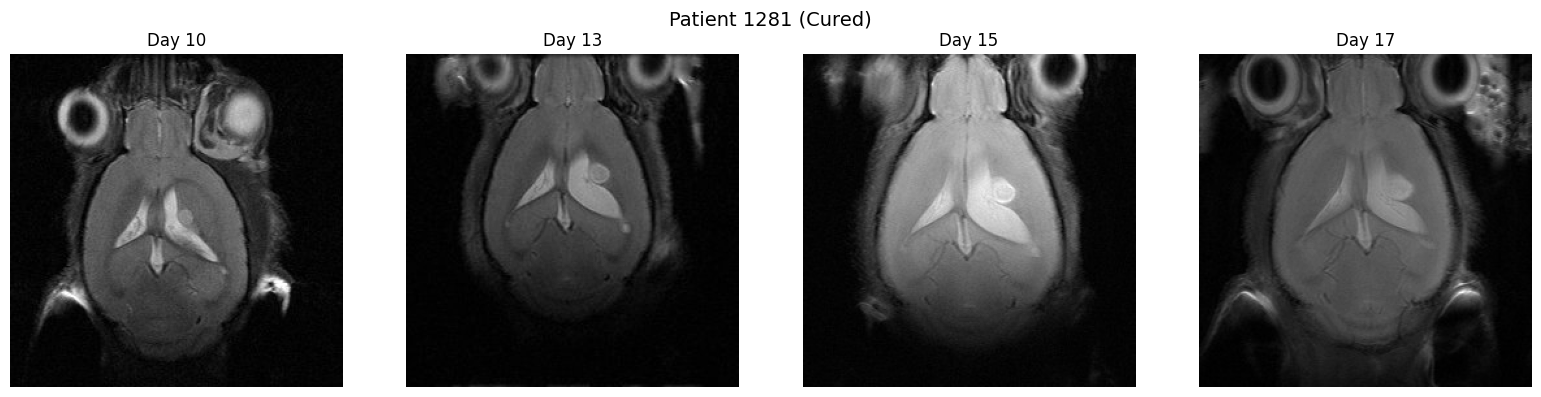
\includegraphics[width=\linewidth]{images/1281_ev.png}
\caption{Longitudinal T2-weighted MRI examinations.}
\label{fig:longitudinal_mri}
\end{subfigure}

\vspace{2mm}

\begin{subfigure}[b]{\textwidth}
\centering
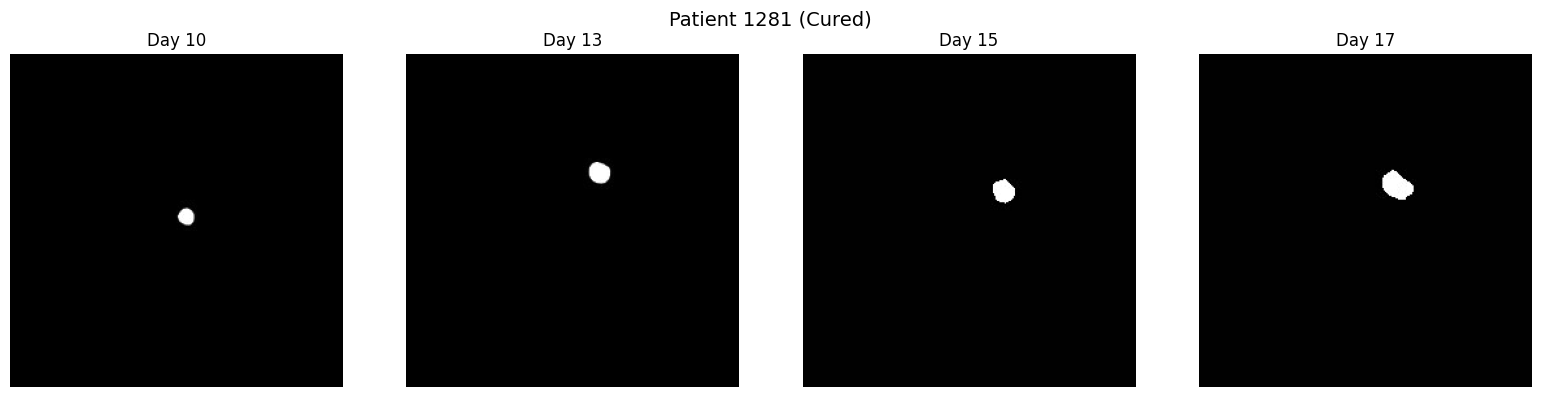
\includegraphics[width=\linewidth]{images/1281_mask_ev.png}
\caption{Corresponding expert tumor segmentation masks.}
\label{fig:longitudinal_mask}
\end{subfigure}
\caption{Illustration of the longitudinal nature of the dataset for a representative treated (cured) animal (subject C1281). (a) Consecutive T2-weighted MRI examinations acquired at different days along tumor evolution and treatment, and (b) their corresponding manually delineated binary tumor masks. Each animal contributes several such examinations acquired at irregular time points, which are treated as individual observations rather than as a jointly modeled temporal sequence.}
\label{fig:longitudinal}
\end{figure}

\begin{table}[H]
\centering
\begin{tabular}{lccc}
\hline
Group & Mice & MRI Examinations & Outcome \\
\hline
Control & 8 & 36 & Natural progression \\
Relapsing & 5 & 84 & Initial response followed by recurrence \\
Cured & 5 & 49 & Complete response \\
\hline
Total & 18 & 169 & -- \\
\hline
\end{tabular}
\caption{Summary of the experimental cohort. MRI examinations correspond to longitudinal imaging sessions acquired throughout tumor evolution. A detailed per-subject breakdown is available in Supplementary Table S1.}
\label{tab:cohort}
\end{table}

\subsection{Study Design and Longitudinal Data Handling}

Although the dataset is longitudinal, complete temporal sequences were not modeled jointly as a multivariate time series \cite{Prinzi2024}. Instead, each imaging time point was treated as an individual labeled observation. Temporal context is preserved through the subject-aware cross-validation scheme (GLOO), which ensures that all examinations from a given animal are withheld together during evaluation, and through a post-hoc temporal analysis of predictive performance stratified by day of study. This design reflects the heterogeneous and irregular sampling of the cohort, in which the number and timing of examinations vary substantially across subjects.

\subsection{Radiomics-Based Pipeline}

The radiomics workflow was designed to transform longitudinal MRI examinations into a structured set of quantitative descriptors capable of capturing tumor morphology, intensity characteristics, and intratumoral heterogeneity throughout treatment. Given the limited sample size and high dimensionality of the feature space, particular emphasis was placed on robust preprocessing, dimensionality reduction, and model regularization to minimize overfitting and maximize generalization.

\subsubsection{Image Preprocessing}

Prior to feature extraction, all MRI scans underwent a standardized preprocessing procedure implemented according to recommendations from the Image Biomarker Standardization Initiative (IBSI) \cite{Zwanenburg_2020}. Intensity normalization was performed to reduce acquisition-related variability and improve reproducibility across imaging sessions. A fixed gray-level discretization bin width of 1 was applied to ensure consistency in texture calculations. To comply with PyRadiomics \cite{pyradiomics} requirements and avoid negative intensity values, a voxel array shift of +1000 was introduced. Extreme intensity values corresponding to potential imaging artifacts were trimmed using a three-standard-deviation threshold. To ensure spatial consistency between subjects and acquisition sessions, all images were resampled to an isotropic in-plane resolution of 0.2 mm using B-spline interpolation. Tumor masks were corrected when necessary and padded with a five-voxel margin to preserve relevant contextual information surrounding the lesion. Finally, images were cropped around the tumor region to reduce computational requirements while maintaining biologically relevant tissue information.

\subsubsection{Radiomic Feature Extraction}

Radiomic features were extracted using the PyRadiomics framework from manually segmented tumor regions on T2-weighted MRI slices. A total of 1,218 quantitative features were computed for each image, including first-order statistics, shape-based descriptors, and second- and higher-order texture features (GLCM, GLRLM, GLSZM, GLDM, and NGTDM). Feature extraction was performed not only on the original MRI images but also on multiple transformed representations, including Laplacian-of-Gaussian (LoG) filtered images at multiple scales ($\sigma = 1.0$, $2.0$, and $3.0$), one-level wavelet decompositions, gradient images, and intensity transformations (square, square-root, logarithmic, and exponential). A complete description of the feature families and image transformations is provided in Supplementary Methods S4.

\subsubsection{Feature Selection and Dimensionality Reduction}

\textcolor{red}{Given the extremely high dimensionality of the radiomic feature space relative to the number of available subjects, a rigorous multi-stage feature selection strategy was implemented entirely within the training partition of each GLOO fold, so that no information from the held-out test animal was used at any selection step. First, missing values were imputed using mean-value substitution. Then, features exhibiting near-zero variance (variance $<0.01$) were removed. Redundancy was then reduced through correlation filtering using Spearman rank correlation coefficients computed on training data only: when two features exhibited a correlation magnitude greater than 0.95, one of them was discarded. Subsequently, statistical filtering was performed using the Mann-Whitney U test on training labels only, retaining features with $p < 0.05$; this non-parametric test was selected because most radiomic variables deviated substantially from normality. Finally, a heuristic filter was applied to retain only features derived from the original (unfiltered) MRI images, excluding those computed from transformed representations (wavelets, Laplacian-of-Gaussian, and intensity transformations), to reduce filter-induced feature redundancy. The resulting feature subset was then applied to the test partition, and all subsequent steps (z-score normalization via a StandardScaler, SMOTE oversampling, and XGBoost training) were fitted exclusively on training data within each fold.}

\subsubsection{Classification Using XGBoost}

The final classification stage was performed using eXtreme Gradient Boosting (XGBoost) \cite{Chen2016}, an ensemble learning algorithm based on gradient-boosted decision trees. XGBoost was selected because it is particularly well-suited to radiomics applications characterized by structured tabular data, limited sample sizes, high-dimensional feature spaces, and complex non-linear interactions among variables. Its built-in L1 and L2 regularization, shrinkage, column subsampling, and tree pruning mechanisms reduce overfitting risk in small datasets, while feature importance scores enable biological interpretation of the resulting models.

Hyperparameter optimization was conducted through grid search embedded within the training procedure. The final configuration is summarized in Supplementary Table~S3, and the complete search grid is reported in Supplementary Table~S2. To address class imbalance between cured and relapsing mice, several resampling strategies were investigated, including the Synthetic Minority Over-sampling Technique (SMOTE) \cite{Chawla2002}, Edited Nearest Neighbors (ENN) \cite{Wilson1972}, and training on the original class distribution. Comparative evaluation demonstrated that controlled oversampling improved sensitivity for the minority cured class while preserving overall model discrimination.


\subsection{Deep Learning-Based Pipeline}

While radiomics relies on handcrafted descriptors, DL enables the automatic extraction of hierarchical feature representations directly from imaging data. This capability is particularly relevant in glioblastoma, where treatment response may be encoded through complex spatial patterns that cannot be fully captured by manually engineered features. Because the application of DL in preclinical imaging is constrained by the limited number of available subjects, a transfer learning strategy was adopted to reduce the risk of overfitting. Additional architectural details are provided in Supplementary Methods S1.

\subsubsection{Image Preparation and Preprocessing}

Each MRI examination consisted of a T2-weighted image together with its corresponding manually delineated tumor mask. Prior to network training, images were resized to the input resolution required by the network while preserving anatomical proportions, and intensity values were normalized to match the distribution expected by ImageNet-pretrained models. Data augmentation (random rotations, horizontal and vertical translations, zoom operations, and intensity perturbations) was applied during training to increase dataset diversity and improve generalization. Control cases were excluded from training, as untreated animals do not reflect the therapeutic dynamics under study. To handle the dataset efficiently, all samples were converted to the TFRecord format and processed through a TensorFlow \texttt{tf.data} pipeline enabling on-the-fly augmentation, shuffling, batching, and prefetching.

\subsubsection{EfficientNetB0 Architecture and Transfer Learning}

The backbone architecture was EfficientNetB0, a CNN proposed by Tan and Le \cite{tan2020efficientnetrethinkingmodelscaling} that employs a compound scaling strategy jointly optimizing network depth, width, and input resolution. EfficientNetB0 was selected because it provides competitive accuracy with only approximately 5.3 million trainable parameters, substantially fewer than architectures such as VGG16, ResNet50, or DenseNet121, which is advantageous in small medical imaging datasets. The network was initialized with ImageNet weights \cite{deng2009}. Initially, the convolutional backbone was frozen, allowing only the classification head to learn task-specific representations; subsequently, the upper layers were unfrozen and fine-tuned with a reduced learning rate, adapting the model to glioblastoma MRI characteristics while preserving robust low-level representations.

\subsubsection{Fine-Tuning Procedure}

Fine-tuning replaced the original ImageNet classification head with a custom binary classification head discriminating between cured and relapsing mice. The last 50 layers of the backbone were unfrozen, the model accepted three-channel input images, and the classification head consisted of a global pooling layer, a dense layer, batch normalization, dropout, and a final sigmoid activation. Training used a binary cross-entropy loss and the Adam optimizer, with a batch size of 32 and random oversampling of the minority class applied only to the training partition within each fold to avoid information leakage. \textcolor{red}{Each fold model was trained for a fixed 20 epochs with no early stopping and no model checkpoint selection based on validation performance; the weights at the final epoch were used for evaluation. Although the held-out test animal's data were passed as \texttt{validation\_data} during training for monitoring purposes only, they did not influence any model-selection or stopping decision.} Dropout regularization was used to reduce overfitting. \textcolor{red}{All experiments were conducted with a fixed random seed (42) applied to Python, NumPy, TensorFlow, and XGBoost, and GPU operation determinism was enforced (\texttt{tf.config.experimental.enable\_op\_determinism()}) to ensure full reproducibility of reported results.} The full fine-tuning configuration is summarized in Supplementary Table~S4.


\subsubsection{Input Configurations}

To investigate the contribution of explicit tumor localization information, two input configurations were evaluated. In the first, the network received only the grayscale T2-weighted MRI image, allowing it to autonomously identify relevant anatomical structures. In the second, manually generated tumor masks were incorporated as additional image channels, explicitly guiding the network toward the lesion. Comparing both configurations enabled assessment of whether prior anatomical knowledge improves predictive performance or whether the network can independently identify the most informative regions.

\subsection{Evaluation and Interpretability}

\subsubsection{Performance Metrics}

Model performance was assessed using a comprehensive set of complementary metrics. The primary metric was the AUC, which measures discrimination between cured and relapsing mice independently of any specific decision threshold. In addition, Accuracy, Sensitivity (recall of the cured class), Specificity, Positive Predictive Value (PPV), Negative Predictive Value (NPV), and F1-score were computed. \textcolor{red}{All metrics were computed at two levels: \textit{exam level}, pooling predictions from all GLOO folds across individual MRI examinations (N=298), and \textit{animal level}, aggregating exam-level predictions per subject via majority vote and computing metrics over the 10 treated animals. Bootstrap 95\% confidence intervals (10\,000 resamples) were computed for exam-level metrics to quantify estimation uncertainty arising from the small effective sample size.} Because the cured and relapsing groups were not perfectly balanced, sensitivity was considered of special interest, as failing to identify a truly responding subject may have important implications for treatment assessment and biomarker discovery.

\subsubsection{Validation Strategy}

A GLOO cross-validation framework was employed for both pipelines. In longitudinal imaging studies, multiple MRI examinations are acquired from the same animal, so observations from the same mouse exhibit substantial intra-subject correlation and cannot be considered statistically independent; random train-test splitting would therefore introduce severe information leakage. To avoid this, all MRI examinations corresponding to a given mouse were assigned exclusively to either the training or testing set within each fold, and one complete animal was withheld for testing at every iteration. Performance values were aggregated across all folds to obtain robust estimates and reduce dependence on any individual animal.

\subsubsection{Temporal Evaluation}

Beyond global performance, predictive behavior was analyzed as a function of tumor evolution time, since treatment-induced imaging changes emerge progressively after therapy administration. Particular attention was devoted to the period between treatment initiation and the onset of visible tumor regression, which represents the most clinically relevant prediction window, as conventional radiological assessment often remains inconclusive during early treatment stages.

\subsubsection{Interpretability Analysis}

Interpretability analyses were conducted for both paradigms. For the radiomics pipeline, feature importance values extracted from the XGBoost classifier were averaged across cross-validation folds to obtain a robust ranking of predictive biomarkers, and the temporal evolution of the most influential features was analyzed to characterize differences between cured and relapsing tumors. For the DL framework, Grad-CAM \cite{selvaraju2017gradcam} was used to generate class-specific attention maps for both correctly classified and misclassified cases, enabling investigation of whether network decisions were based on biologically meaningful tumor regions. Additional methodological details of Grad-CAM are provided in Supplementary Methods S3.

\section*{Data availability}
The dataset analyzed during the current study was sourced from previously published experiments and is available from the corresponding author upon reasonable request.

\section*{Acknowledgements}
The authors thank the joint preclinical MRI facility of the Universitat Autònoma de Barcelona and the Centro de Investigación Biomédica en Red-Bioingeniería, Biomateriales y Nanomedicina (CIBER-BBN), where all MRI experiments were carried out, as part of Unit 25 of NANBIOSIS (Cerdanyola del Vallès, Spain).

\section*{Author contributions}
J.G.: conceptualization, methodology, software, formal analysis, investigation, data curation, visualization, and writing of the original draft.\newline
A.P.C.: conceptualization, data acquisition, supervision, funding acquisition, manuscript review and editing.\newline
A.V.: conceptualization, methodology, supervision, funding acquisition, manuscript review and editing.

\section*{Funding}
This work was funded by MICIU/AEI/10.13039/501100011033/ (grants PID2023-147750NB-I00 to A.P.C. and PID2022-143299OB-I00 to A.V.), Generalitat de Catalunya (2021 SGR 0135), and Instituto de Salud Carlos III (CIBER-BBN group CB06-01-0010).

\section*{Competing interests}
The authors declare no competing interests.

\section*{Additional information}
\textbf{Supplementary information} accompanies this manuscript, comprising Supplementary Methods, Supplementary Tables S1--S5, and Supplementary Figures S1--S5.

% --- BIBLIOGRAFÍA ---
\bibliographystyle{unsrt}
\bibliography{refs}


\end{document}